% kernel_cut.tex — ONE source, ONE rendered SVG (kernel_cut.svg), embedded in ../concurrent_layers.md.
%
% The kernel-scale twin of system_cut.tex: mem_copy as an HwSystem with NO crossbar.  The DUT is the
% kernel alone -- a composite of three tasks -- in one sub-top; the testbench is the command driver,
% the completion sink and the memory model, each answering ports that leave the top.  Same palette
% and scopes as system_cut.tex, so the two pictures read with one legend.
%
% Render: bash render.sh   (MiKTeX pdflatex -> PDF -> dvisvgm --pdf -> SVG)
\documentclass[tikz,border=6pt]{standalone}
\usepackage{tikz}
\usetikzlibrary{arrows.meta,positioning,calc,fit,backgrounds}

\definecolor{hlsfill}{HTML}{DCE9F7}  \definecolor{hlsline}{HTML}{2C6FB5}   % Vitis HLS -> csynth
\definecolor{rtlfill}{HTML}{DFF0D8}  \definecolor{rtlline}{HTML}{3C7A2E}   % hand-written RTL leaf
\definecolor{ipfill}{HTML}{EADCF2}   \definecolor{ipline}{HTML}{7A4A9A}    % vendor IP (create_ip)
\definecolor{tbfill}{HTML}{F2E6D0}   \definecolor{tbline}{HTML}{9A6B1F}    % testbench C++ model
\definecolor{dutline}{HTML}{1F3B5C}
\definecolor{devline}{HTML}{555555}
\definecolor{sysline}{HTML}{8A8A8A}
\definecolor{inkgray}{HTML}{444444}

\begin{document}
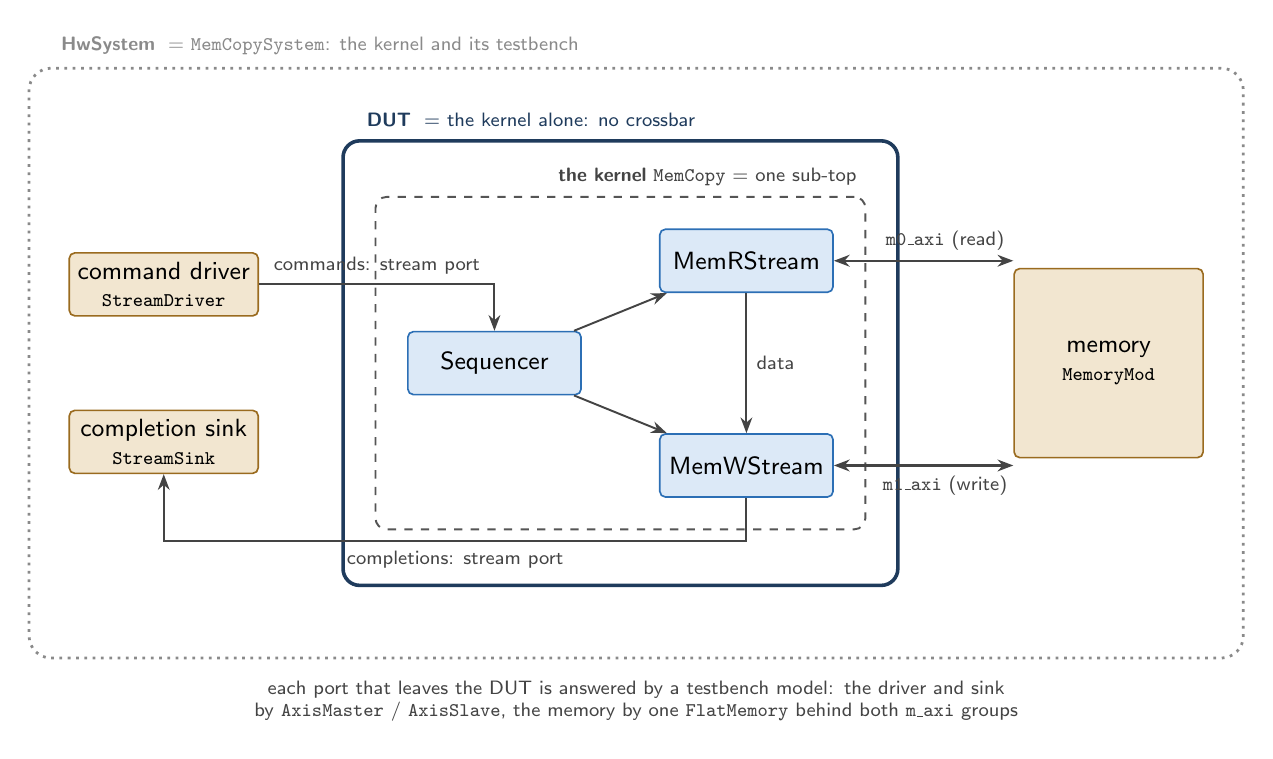
\begin{tikzpicture}[
  font=\sffamily\small,
  blk/.style   = {draw, rounded corners=2pt, minimum height=8mm, align=center, line width=0.6pt,
                  inner sep=2pt},
  hls/.style   = {blk, fill=hlsfill, draw=hlsline, minimum width=22mm},
  tb/.style    = {blk, fill=tbfill, draw=tbline, minimum width=24mm},
  data/.style  = {-{Stealth[length=2mm]}, line width=0.7pt, draw=inkgray},
  axi/.style   = {{Stealth[length=2mm]}-{Stealth[length=2mm]}, line width=0.9pt, draw=inkgray},
  device/.style= {draw=devline, dashed, rounded corners=4pt, line width=0.7pt},
  dut/.style   = {draw=dutline, rounded corners=6pt, line width=1.3pt},
  sys/.style   = {draw=sysline, dotted, rounded corners=8pt, line width=1.0pt},
  lbl/.style   = {font=\sffamily\scriptsize, text=inkgray},
  tag/.style   = {font=\sffamily\scriptsize\bfseries},
]

% ---------------- the kernel: a composite of three tasks (Vitis HLS) -------------------------
\node[hls] (seq) at (4.2,  0.0) {Sequencer};
\node[hls] (rd)  at (7.4,  1.3) {MemRStream};
\node[hls] (wr)  at (7.4, -1.3) {MemWStream};
\draw[data] (seq) -- (rd);
\draw[data] (seq) -- (wr);
\draw[data] (rd) -- node[lbl, right] {data} (wr);
\begin{scope}[on background layer]
  \node[device, fit=(seq)(rd)(wr), inner sep=4mm] (dev) {};
\end{scope}
\node[lbl, anchor=south east] at (dev.north east) {\textbf{the kernel} \texttt{MemCopy} = one sub-top};

\begin{scope}[on background layer]
  \node[dut, fit=(dev), inner xsep=4mm, inner ysep=7mm] (dut) {};
\end{scope}
\node[tag, text=dutline, anchor=south west] at ($(dut.north west)+(2mm,0.3mm)$)
     {DUT \;\textmd{= the kernel alone: no crossbar}};

% ---------------- the testbench -----------------------------------------------------------------
\node[tb] (drv)  at (0.0,  1.0) {command driver\\[-1pt]\scriptsize\texttt{StreamDriver}};
\node[tb] (sink) at (0.0, -1.0) {completion sink\\[-1pt]\scriptsize\texttt{StreamSink}};
\node[tb, minimum height=24mm] (mem) at (12.0, 0.0) {memory\\[-1pt]\scriptsize\texttt{MemoryMod}};

\draw[data] (drv.east) -| node[lbl, above, pos=0.25] {commands: stream port} (seq.north);
\draw[data] (wr.south) -- ++(0,-0.55) -| node[lbl, below, pos=0.25] {completions: stream port} (sink.south);
\draw[axi]  (rd.east) -- node[lbl, above, pos=0.62] {\texttt{m0\_axi} (read)} (mem.west |- rd.east);
\draw[axi]  (wr.east) -- node[lbl, below, pos=0.62] {\texttt{m1\_axi} (write)} (mem.west |- wr.east);

\begin{scope}[on background layer]
  \node[sys, fit=(drv)(sink)(mem)(dut), inner xsep=5mm, inner ysep=9mm] (sys) {};
\end{scope}
\node[tag, text=sysline, anchor=south west] at ($(sys.north west)+(3mm,0.3mm)$)
     {HwSystem \;\textmd{= \texttt{MemCopySystem}: the kernel and its testbench}};
\node[lbl, align=center, anchor=north, text width=120mm] at ($(sys.south)+(0,-0.15)$)
     {each port that leaves the DUT is answered by a testbench model:
      the driver and sink by \texttt{AxisMaster} / \texttt{AxisSlave},
      the memory by one \texttt{FlatMemory} behind both \texttt{m\_axi} groups};

\end{tikzpicture}
\end{document}
